\chapter{Szimulációk, eredmények}

\section{Súlyzó gráf}

Például egy súlyzó gráfról a következő képek készültek:

\begin{figure}[H]
  \centering
  \begin{subfigure}{.3\linewidth}
    \centering
    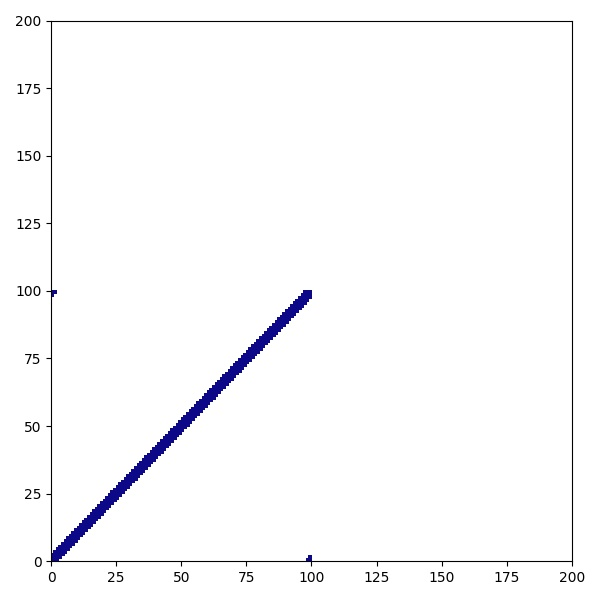
\includegraphics[width=\linewidth]{./figures/sulyzo/subgraph_00.jpg}
    \caption{Bal kör}
    \label{fig:sub1}
  \end{subfigure}
  \begin{subfigure}{.3\linewidth}
    \centering
    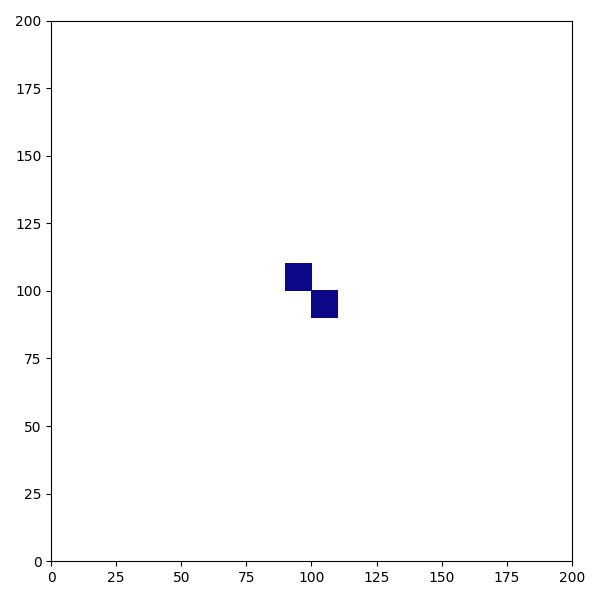
\includegraphics[width=\linewidth]{./figures/sulyzo/subgraph_02.jpg}
    \caption{Középső teljes páros gráf}
    \label{fig:sub2}
  \end{subfigure}
  \begin{subfigure}{.3\linewidth}
    \centering
    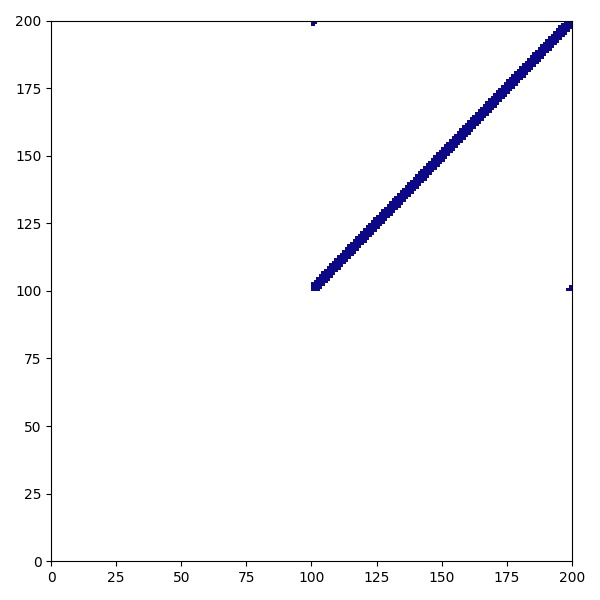
\includegraphics[width=\linewidth]{./figures/sulyzo/subgraph_01.jpg}
    \caption{Jobb kör}
    \label{fig:sub3}
  \end{subfigure}
  \caption{Súlyzó gráf részgráfjai}
  \label{fig:all}
\end{figure}

\begin{figure}[H]
  \centering
  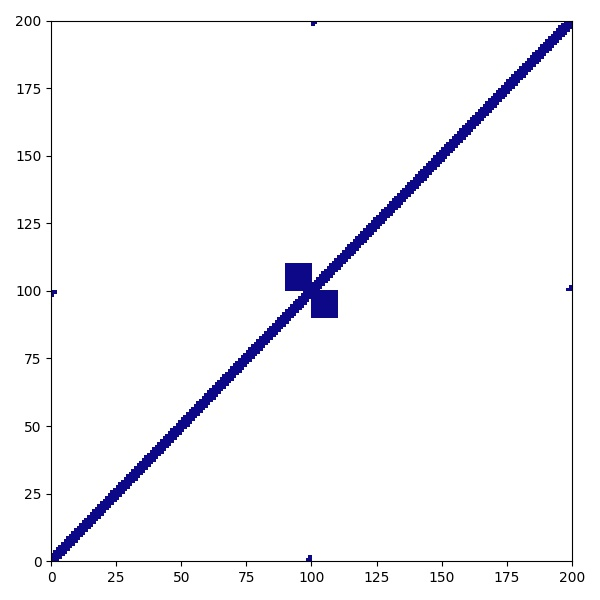
\includegraphics[width=0.5\linewidth]{./figures/sulyzo/graph.jpg}
  \caption{Súlyzó gráf}
\end{figure}

\begin{figure}[H]
  \centering
  \begin{subfigure}{.45\linewidth}
    \centering
    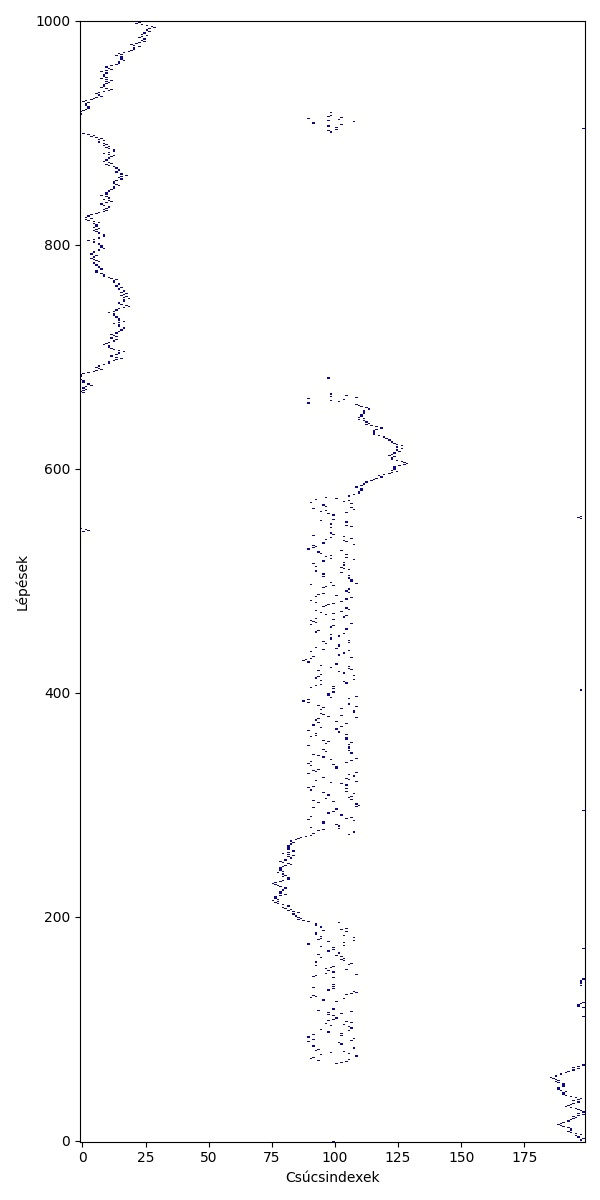
\includegraphics[width=\linewidth]{./figures/sulyzo/sim00.jpg}
    \caption{1 bolyongó}
  \end{subfigure}
  \begin{subfigure}{.45\linewidth}
    \centering
    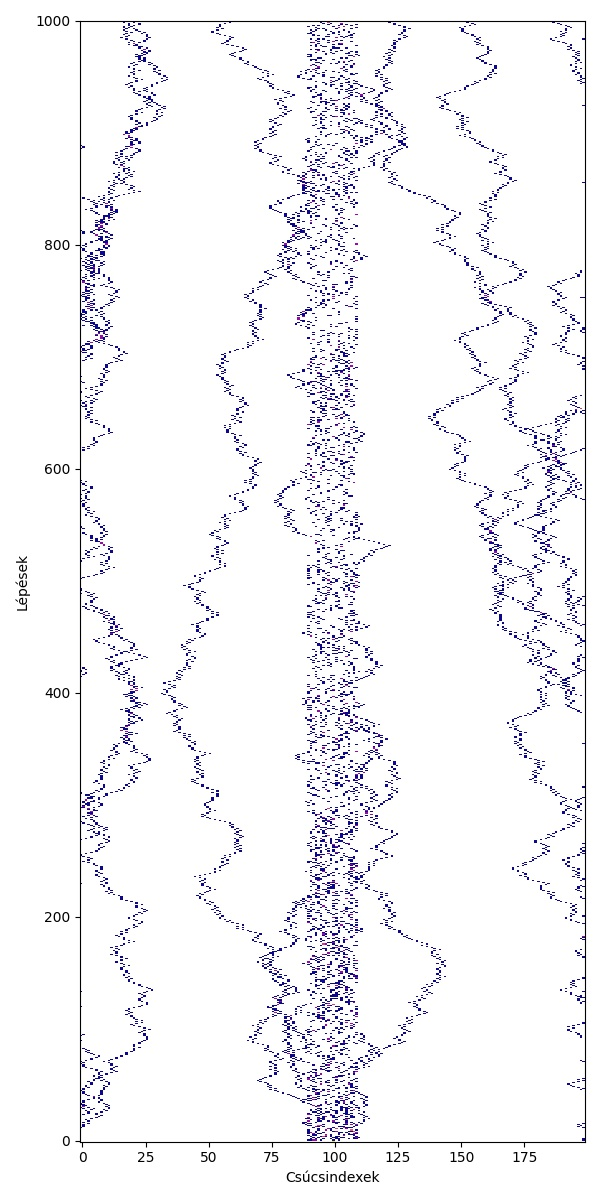
\includegraphics[width=\linewidth]{./figures/sulyzo/sim01.jpg}
    \caption{10 bolyongó}
  \end{subfigure}
\end{figure}

\begin{figure}[H]
  \centering
  \begin{subfigure}{.45\linewidth}
    \centering
    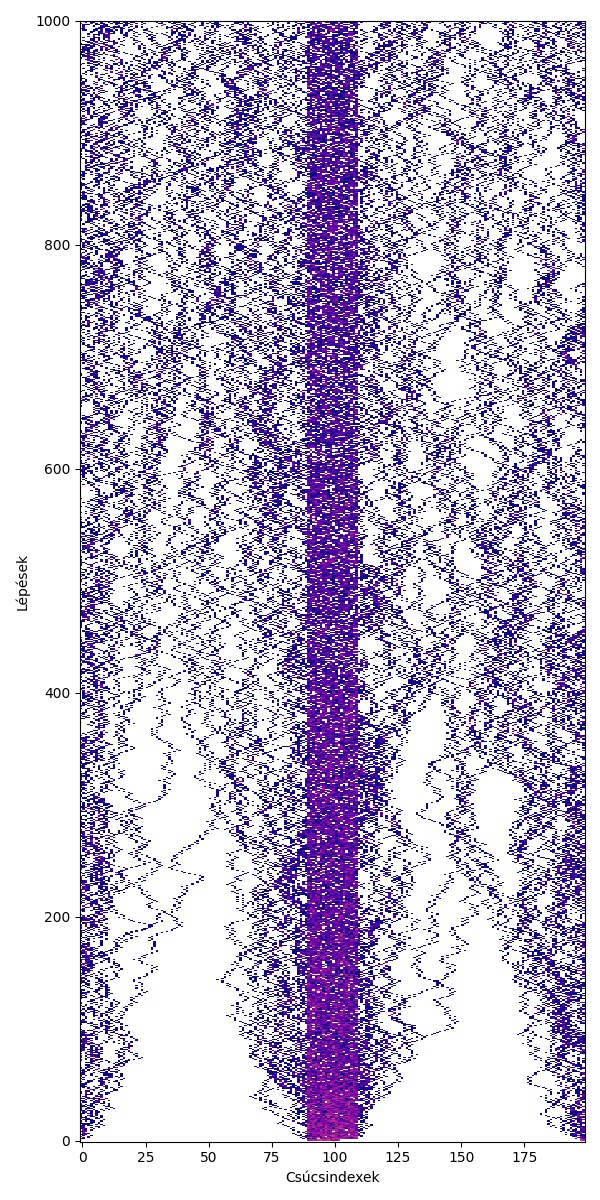
\includegraphics[width=\linewidth]{./figures/sulyzo/sim02.jpg}
    \caption{100 bolyongó}
  \end{subfigure}
  \begin{subfigure}{.45\linewidth}
    \centering
    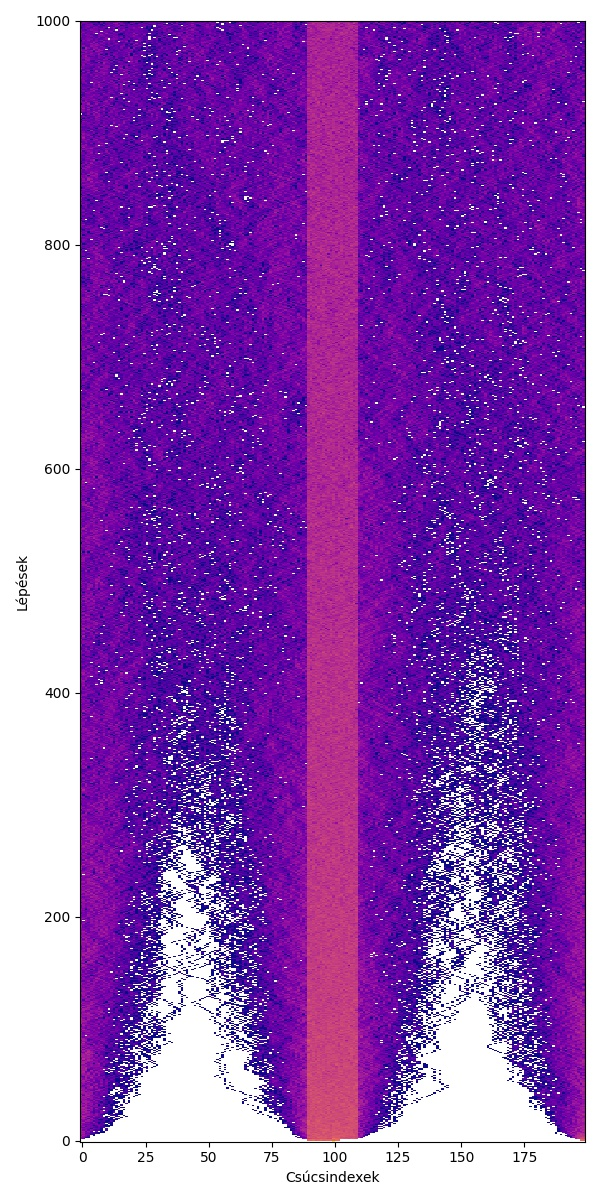
\includegraphics[width=\linewidth]{./figures/sulyzo/sim03.jpg}
    \caption{1000 bolyongó}
  \end{subfigure}
\end{figure}

\section{Ragasztott bináris gráf}

\begin{figure}[H]
  \centering
  \begin{subfigure}{.3\linewidth}
    \centering
    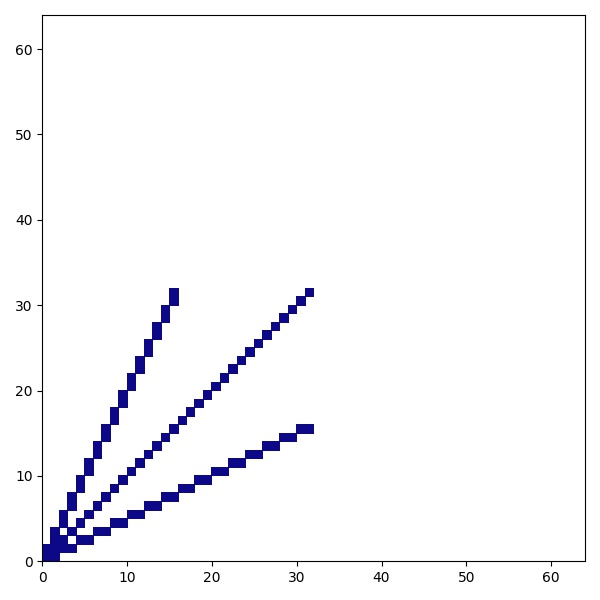
\includegraphics[width=\linewidth]{./figures/ragasztott_binaris/subgraph_00.jpg}
    \caption{Bal bináris fa}
  \end{subfigure}
  \begin{subfigure}{.3\linewidth}
    \centering
    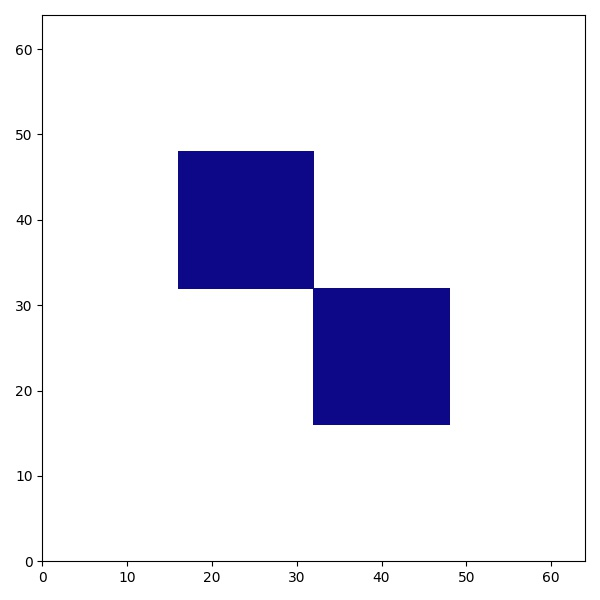
\includegraphics[width=\linewidth]{./figures/ragasztott_binaris/subgraph_02.jpg}
    \caption{Középső teljes páros gráf}
  \end{subfigure}
  \begin{subfigure}{.3\linewidth}
    \centering
    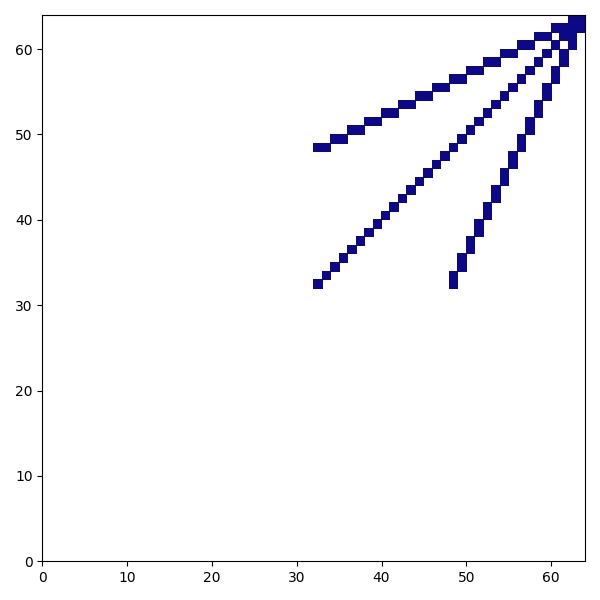
\includegraphics[width=\linewidth]{./figures/ragasztott_binaris/subgraph_01.jpg}
    \caption{Jobb bináris fa}
  \end{subfigure}
  \caption{Ragasztott bináris gráf részgráfjai}
\end{figure}

\begin{figure}[H]
  \centering
  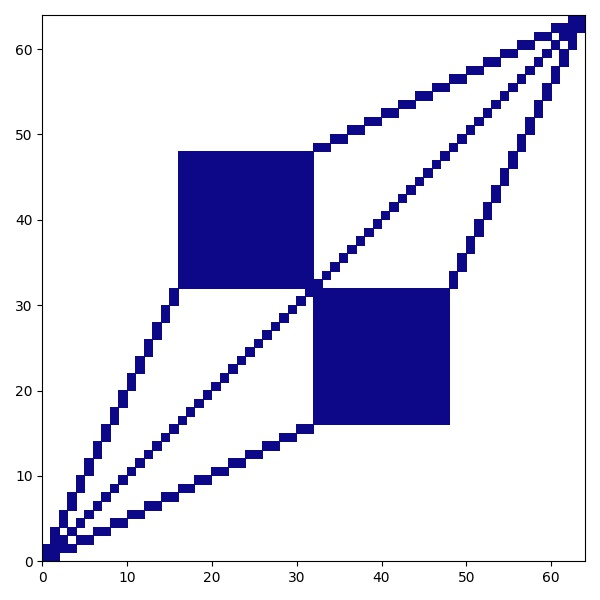
\includegraphics[width=0.5\linewidth]{./figures/ragasztott_binaris/graph.jpg}
  \caption{Ragasztott bináris gráf}
\end{figure}

\begin{figure}[H]
  \centering
  \begin{subfigure}{.45\linewidth}
    \centering
    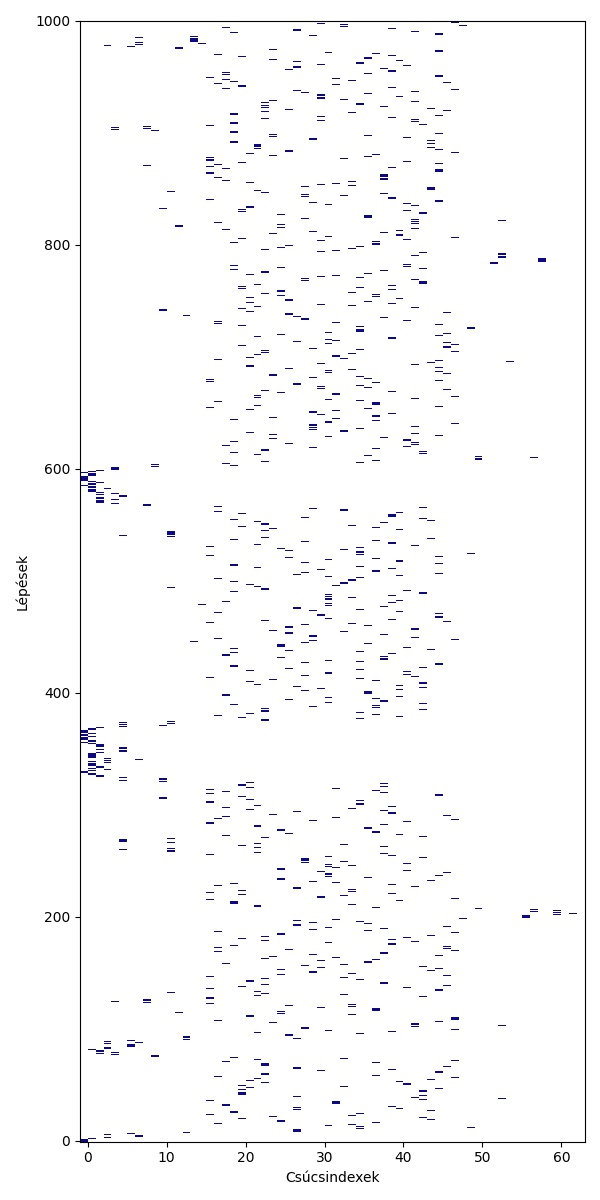
\includegraphics[width=\linewidth]{./figures/ragasztott_binaris/sim00.jpg}
    \caption{1 bolyongó}
  \end{subfigure}
  \begin{subfigure}{.45\linewidth}
    \centering
    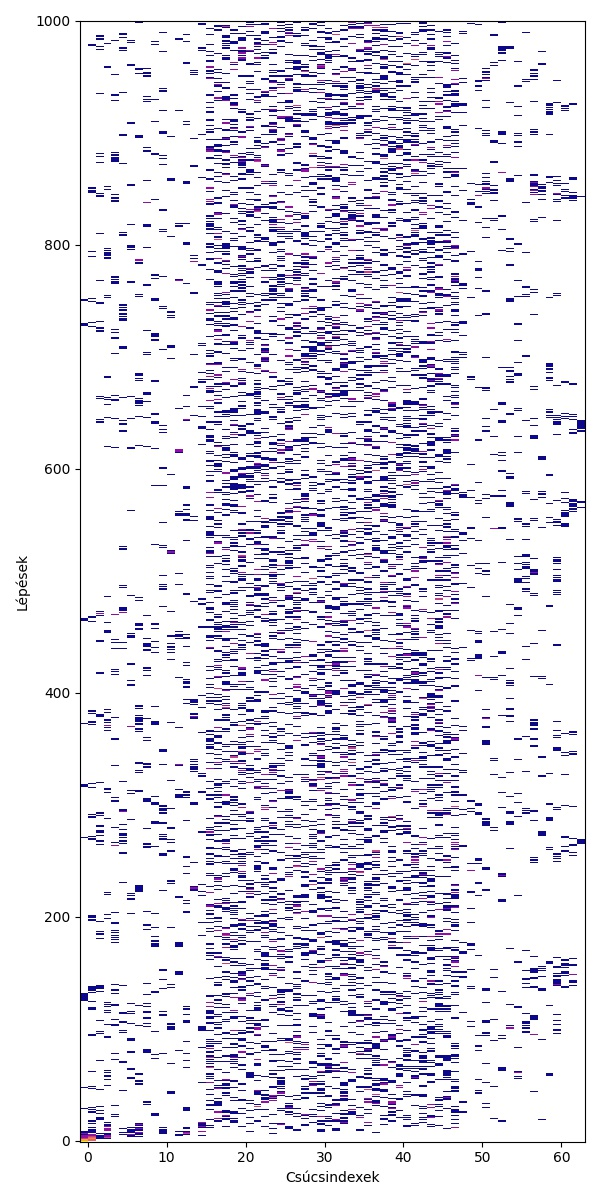
\includegraphics[width=\linewidth]{./figures/ragasztott_binaris/sim01.jpg}
    \caption{10 bolyongó}
  \end{subfigure}
\end{figure}

\begin{figure}[H]
  \centering
  \begin{subfigure}{.45\linewidth}
    \centering
    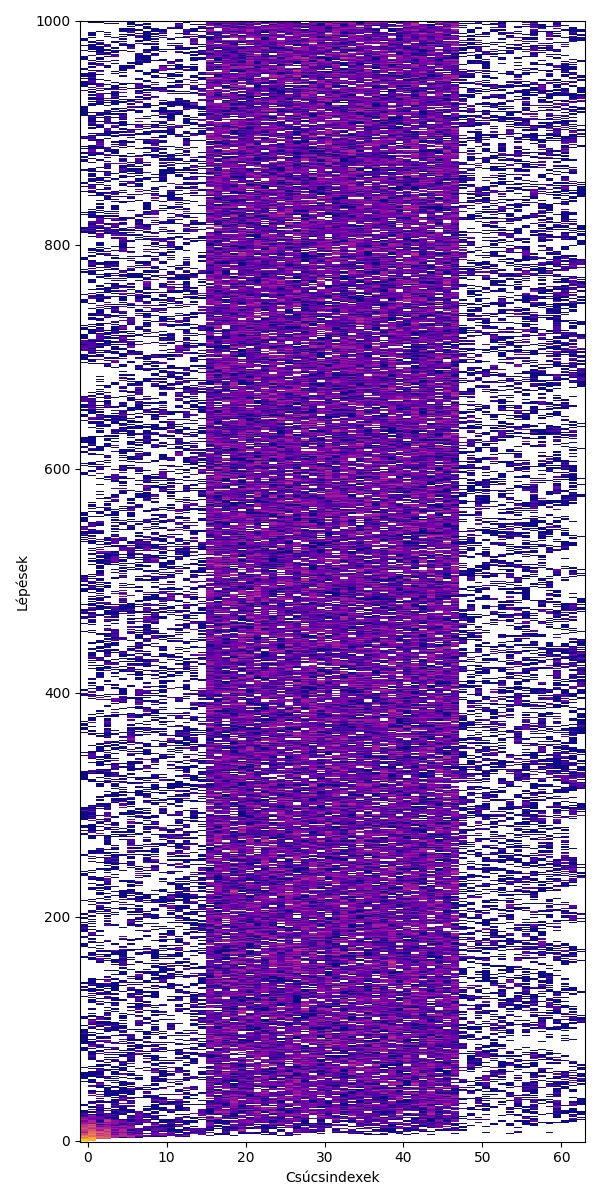
\includegraphics[width=\linewidth]{./figures/ragasztott_binaris/sim02.jpg}
    \caption{100 bolyongó}
  \end{subfigure}
  \begin{subfigure}{.45\linewidth}
    \centering
    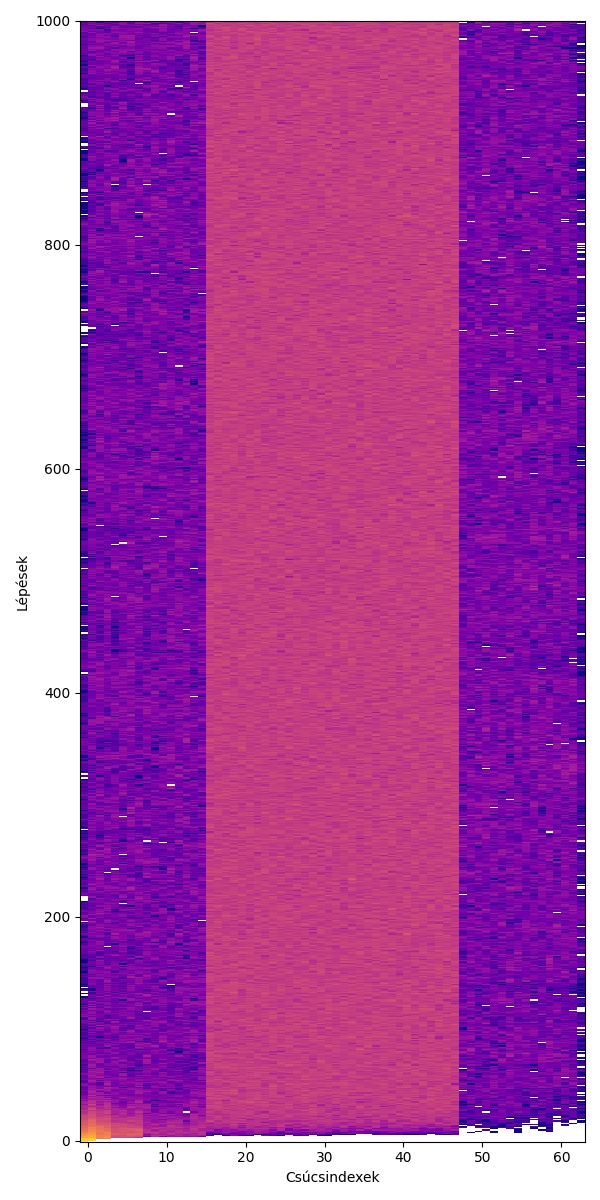
\includegraphics[width=\linewidth]{./figures/ragasztott_binaris/sim03.jpg}
    \caption{1000 bolyongó}
  \end{subfigure}
\end{figure}

